Video notes: vid12.mp4

\subsection*{Example}
Second order example.  N = 2

We expect that poles around the unit circle at $H(s)H(-s)$.

This is the N-even case, so the poles are rotated so you don't get 
poles on the $j\omega$ axis:

We expect the angle to be $3\pi/4$ (see chart)

\paulhint{see frame 17a taken at}\\
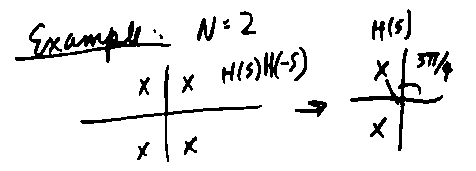
\includegraphics[scale=0.5]{frames/17a}\\

We can express $H(s)$ as a cascade of these poles:


\paulhint{see eqn 17b taken at 1:42}\\
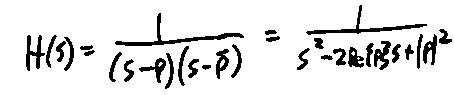
\includegraphics[scale=0.5]{frames/17b}\\

What is P? We can write it as $e^{j3/4\pi}$ which means the real part is
$cos(3\pi/4)$, which is equal to $-1/\sqrt{2}$. 

\paulhint{see eqn + graph 17c taken at 3:38}\\
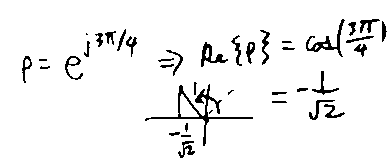
\includegraphics[scale=0.5]{frames/17c}\\

Now that we have found that middle coefficient, we can rewrite 
the transfer function as:

\paulhint{see eqn + graph 17d taken at 4:09}\\
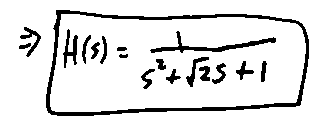
\includegraphics[scale=0.5]{frames/17d}\\

\subsection*{Go Digital}

When you map the splane to the unit circle, the rigthand plane maps
to the exterior unit circle, and the lefthand plane maps to the interior unit circle,
which is only true for $c > 0$, otherwise they change places if it is negative.

\paulhint{LHP and RHP 17e taken at }\\
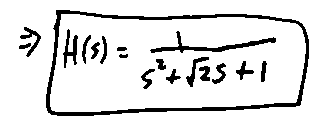
\includegraphics[scale=0.5]{frames/17d}\\

We plug in the bilinear transform to:

\paulhint{17f taken at 6:16}\\
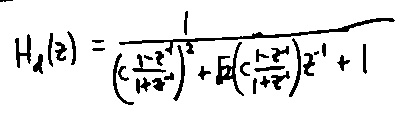
\includegraphics[scale=0.5]{frames/17f}\\

"Unit term" is just one. 

Now we want to get it into a better form. 

First we multiply the numerator by $(1 + z^{-1})^2$:

\paulhint{17g taken at 7:16}\\
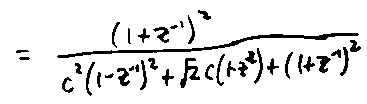
\includegraphics[scale=0.5]{frames/17g}\\

Multiply this out to collect powers of z inverse:

\paulhint{17h taken at }\\
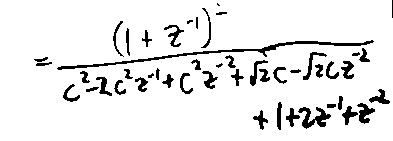
\includegraphics[scale=0.5]{frames/17h}\\

Collect these things together. Find all the constant terms. 

\paulhint{17i taken at 7:16}\\
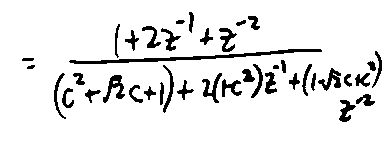
\includegraphics[scale=0.5]{frames/17i}\\

We're still not quite done, becuase we need a monic denominator. So we pull
the first term out to make it a gain:

\paulhint{17j taken at 10:12}\\
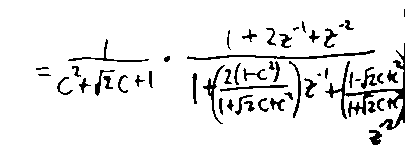
\includegraphics[scale=0.5]{frames/17j}\\

We've done a second order butterworth filter, and we have digitized it.

Now, let's set the cutoff frequency $\omega_c$

\subsection*{Set the cutoff frequency to $\pi/2$}

To do that, we have to normalize it. To do that, you need to look
at the biliear transform mapping:

\paulhint{17k taken at 11:53}\\
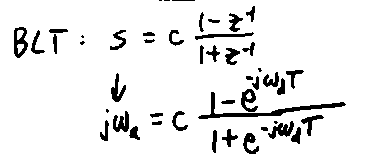
\includegraphics[scale=0.5]{frames/17k}\\

We're normalized, so $\omega_a = 1$. We want $\omega_d T = \pi/2$

This implies $e^{-j\omega_d T} = e^{-j\pi/2} = -j$.

We start with this equation:

\begin{align*}
j\omega_a = c \frac{1 - e^{_j\omega_d T}}{1 + e^{-j \omega_d T}}
\end{align*}

And we factor out just like we did with the simplest lowpass filter:

% \paulhint{17l taken at 13:39}\\
% 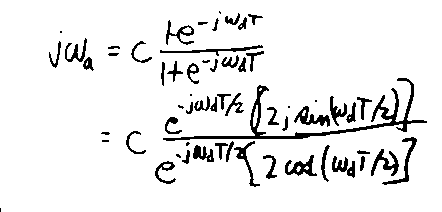
\includegraphics[scale=0.5]{frames/17l}\\
\begin{align*}
    j\omega_a &= 
    c \frac{
        1 - e^{-j\omega_d T}   
    } {
        1 + e^{-j\omega_d T}   
    } \\
    &= 
    c \frac{
        e^{-j \omega_d T / 2} [ 2 j\sin(\omega_d T /2 ) ]
    } {
        e^{-j \omega_d T / 2} [ 2 \cos(\omega_d T / 2) ]
    }
\end{align*}
Our final equation is

\begin{align*}
j\omega_a = c j \tan(\omega_d T / 2)
\end{align*}

This is a nice simple expression to work with, as the j's cancel. 

The analogue frequency axis relates to the digial frequency axis in this way:

\begin{align*}
\omega_a = c \tan(\omega_d T / 2)
\end{align*}

We desire $\omega_a = 1$  to map to $\omega_dT = \pi / 2$, so this all equals
$c \tan(\pi/4) = 1$

Therefore, our halfband lowpass filter (cuts off at half the sampling rate) is:

\begin{align*}
H(z) = \frac{1}{2 + \sqrt{2}} \frac{(1+ z^{-1})^2} {1 + 
(\frac{2 - \sqrt{2}}{2 + \sqrt{2}})z^{-2}
}
\end{align*}

We have two zeros at half the sampling rate, and imaginary poles on the imaginary
axis in the z-plane. This is a butterworth filter that has a -3db at 
$\omega_d  = \pi/2$. 

\paulhint{17m taken at 16:22}\\
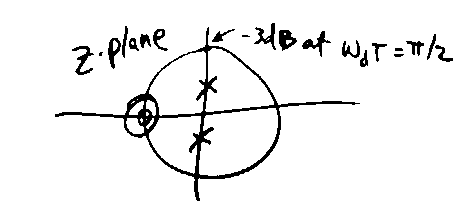
\includegraphics[scale=0.5]{frames/17m}\\

\subsection*{Check our Work}

dc gain = $H_d(1) = \frac{1}{2 + \sqrt{2}} 
\frac{2^2}{1 +
\frac{2 - \sqrt{2}}{2 + \sqrt{2}}
} =
\frac{4}{2 +\sqrt{2} + 2 - \sqrt{2} } = 1
$

DC is one as expected.

Half the sampling rate is easy to check, you plug in -1 and you get two zeros.

You can check that the cutoff freq is exactly -3db:

\paulhint{17n taken at 18:21}\\
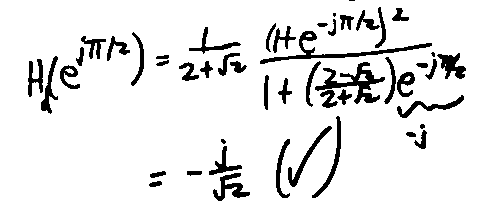
\includegraphics[scale=0.5]{frames/17n}\\

(he skipped a couple of steps here)\\
